\likeechapter{Приложение А}
\appendix
\counterwithout{figure}{chapter}
\setcounter{figure}{0}
\begin{figure}[H]
	\centering
	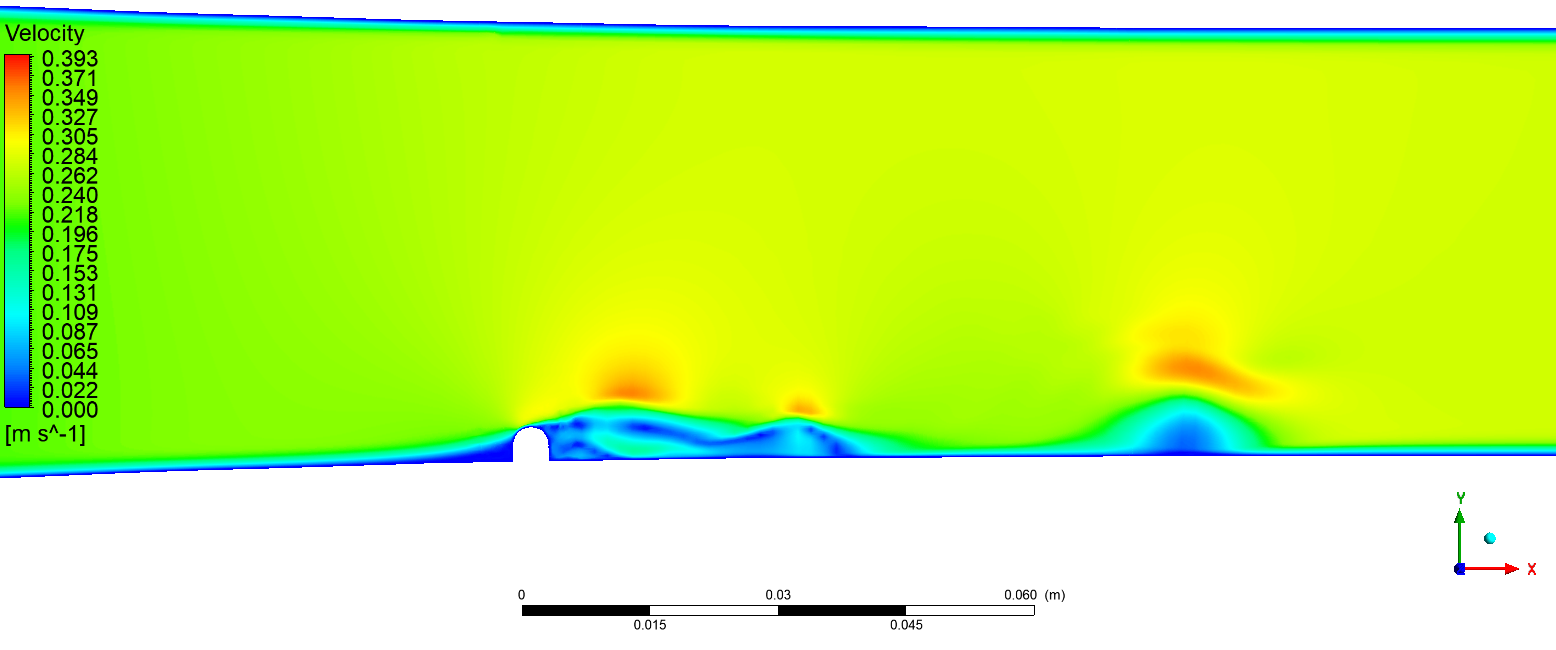
\includegraphics[width=0.9\linewidth]{../Assets/T0_Velocity_ContourXY}
	\caption{PlaneXY, t = 0.6 c}
	\label{fig:t0velocitycontourxy}
\end{figure}
\begin{figure}[H]
	\begin{subfigure}{.5\textwidth}
		\centering
		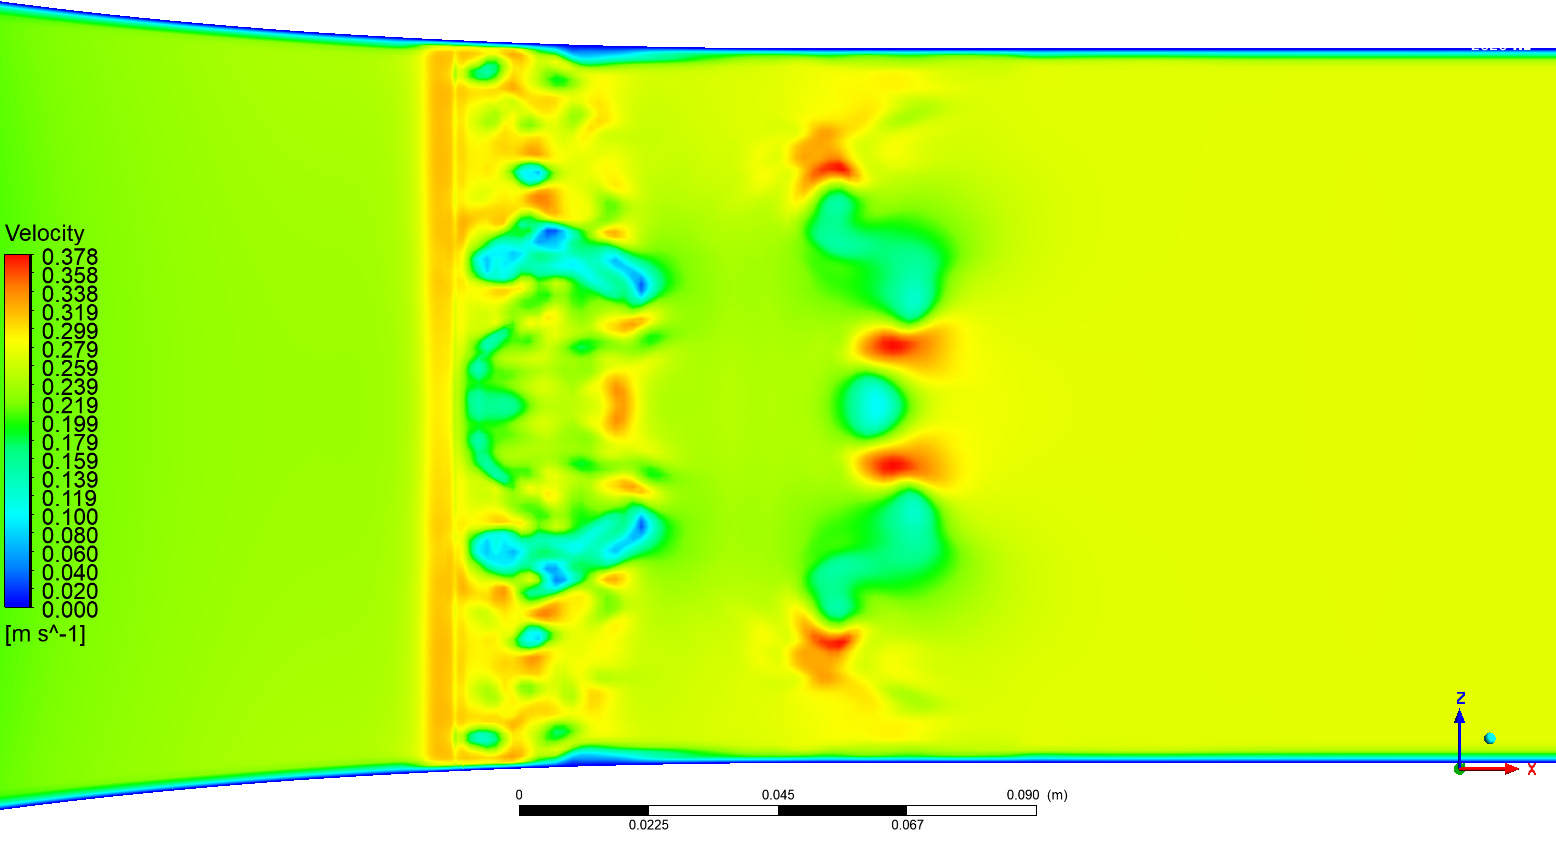
\includegraphics[width=1.7\linewidth, angle=90]{../Assets/T0_Velocity_ContourXZ20M}
		\caption{PlaneXZ20M}
		\label{fig:t0velocitycontourxz20m}
	\end{subfigure}%
	\begin{subfigure}{.5\textwidth}
		\centering
		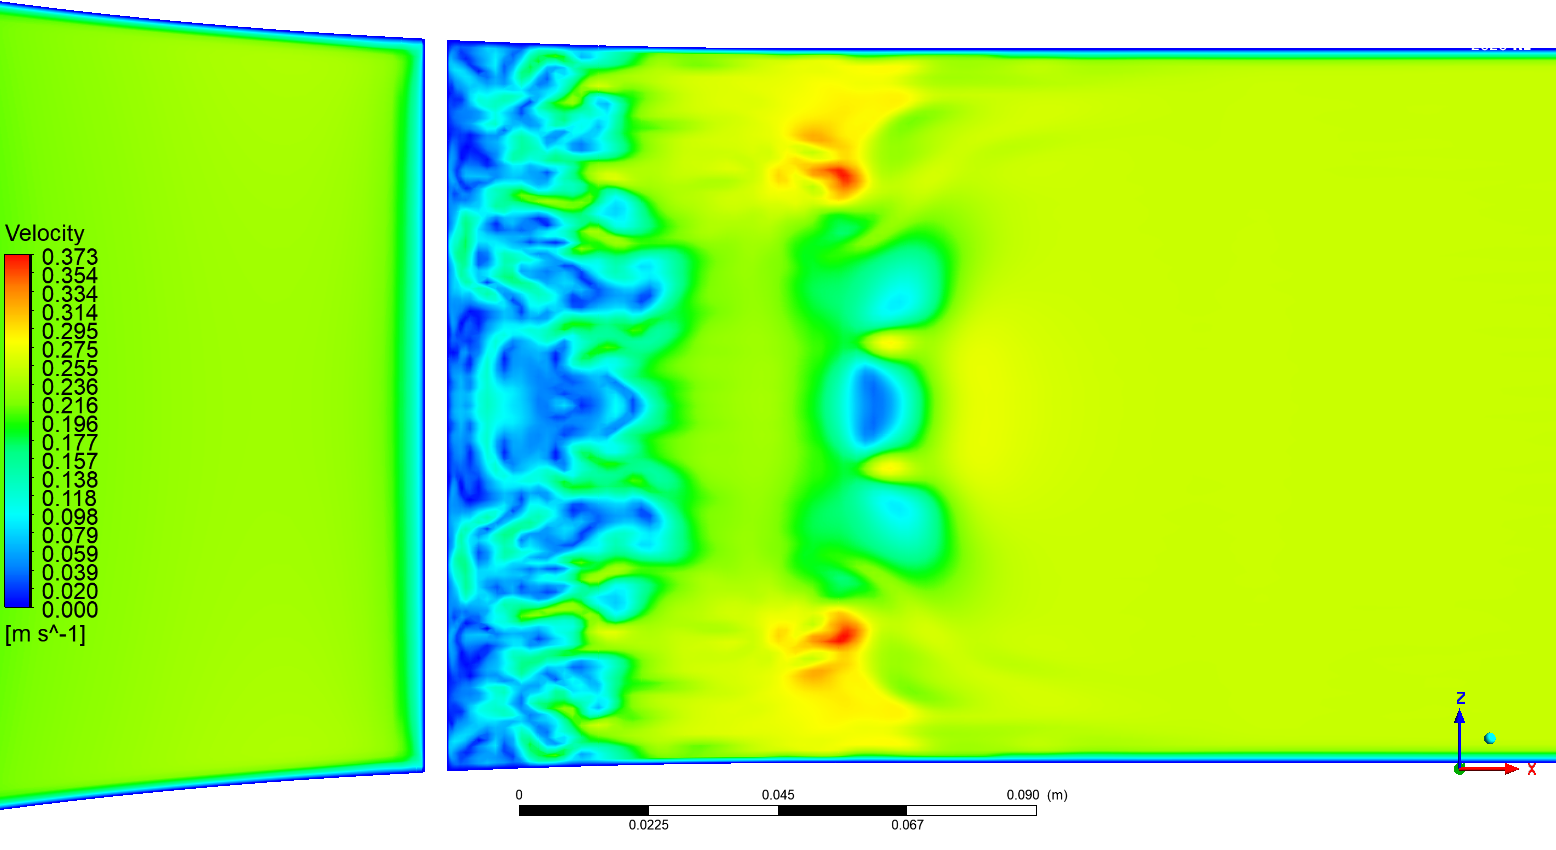
\includegraphics[width=1.7\linewidth, angle=90]{../Assets/T0_Velocity_ContourXZ23M}
		\caption{PlaneXZ23M}
		\label{fig:t0velocitycontourxz23m}
	\end{subfigure}
		\caption{PlaneXZ, t = 0.6 c}
		\label{fig:t0velocitycontourxz}
\end{figure}
\newpage
\begin{flushright}
	\MakeUppercase{\textbf{Приложение А}}
\end{flushright}